\documentclass[12pt,a4paper,fleqn]{article}
\usepackage[utf8]{inputenc}
\usepackage[spanish, mexico]{babel}
\usepackage[spanish]{layout}
\usepackage[article]{ragged2e}
\usepackage[pdftex]{graphicx}
\usepackage{amsmath}
\usepackage{amssymb}
\usepackage{amsthm}
\usepackage{zed-csp}
\usepackage[pdftex,colorlinks,linkcolor=blue]{hyperref}
\usepackage[cm]{fullpage}

\usepackage{titlesec}
\titleclass{\subsubparagraph}{straight}[\subparagraph]
\newcounter{subsubparagraph}
\renewcommand{\thesubsubparagraph}{\Alph{subsubparagraph}}
\titleformat{\subsubparagraph}[runin]{\normalfont\normalsize\bfseries}{\thesubsubparagraph}{1em}{}
\titlespacing*{\subsubparagraph} {\parindent}{3.25ex plus 1ex minus .2ex}{1em}


\newcommand{\modulo}{{\bf Module }}

\newenvironment{module}[1]{\hypertarget{mi:#1}{}\vspace{0.5cm}\noindent\begin{tabular}{|p{0.2\linewidth} p{0.7\linewidth}|} \hline \modulo &{\bf #1} \\}{\hline\end{tabular}\vspace{0.5cm}}

\newenvironment{moduleNODP}[1]{\hypertarget{mi:#1}{}\vspace{0.5cm}\noindent\begin{tabular}{|p{0.2\linewidth} p{0.7\linewidth}|} \hline \modulo &{\bf #1} \\}{\hline\end{tabular}\vspace{0.5cm}}

\newenvironment{gmodule}[2]{\hypertarget{mi:#1}{} \vspace{0.5cm}\noindent\begin{tabular}{|p{0.25\linewidth} p{0.65\linewidth}|} \hline {\bf Generic Module} & {\bf #1(#2)} \\}{\hline\end{tabular}\vspace{0.5cm}}

\newenvironment{gmoduleNODP}[2]{\hypertarget{mi:#1}{} \vspace{0.5cm}\noindent\begin{tabular}{|p{0.25\linewidth} p{0.65\linewidth}|} \hline & \multicolumn{1}{r|}{\hyperlink{mg:#1}{\fbox{MG}}} \\ {\bf Generic Module} & {\bf #1(#2)} \\}{\hline\end{tabular}\vspace{0.5cm}}

\newenvironment{hmodule}[2]{\hypertarget{mi:#1}{} \vspace{0.5cm}\noindent\begin{tabular}{|p{0.2\linewidth} p{0.7\linewidth}|} \hline {\bf Module} & {\bf #1 inherits from} \hyperlink{mi:#2}{#2} \\}{\hline\end{tabular}\vspace{0.5cm}}

\newenvironment{hmoduleNODP}[2]{\hypertarget{mi:#1}{} \vspace{0.5cm}\noindent\begin{tabular}{|p{0.2\linewidth} p{0.7\linewidth}|} \hline & \multicolumn{1}{r|}{\hyperlink{mg:#1}{\fbox{MG}}} \\ {\bf Module} & {\bf #1 inherits from} \hyperlink{mi:#2}{#2} \\}{\hline\end{tabular}\vspace{0.5cm}}

\newcommand{\cmodule}[3]{\hypertarget{mi:#1}{} \vspace{0.5cm}\noindent\begin{tabular}{|p{0.2\linewidth} p{0.7\linewidth}|} \hline {\bf Module} & {\bf #1 is} \hyperlink{mi:#2}{#2}(\hyperlink{mi:#3}{#3})\\ \hline\end{tabular}\vspace{0.5cm}}

\newcommand{\cmoduleNODP}[3]{\hypertarget{mi:#1}{} \vspace{0.5cm}\noindent\begin{tabular}{|p{0.2\linewidth} p{0.7\linewidth}|} \hline & \multicolumn{1}{r|}{\hyperlink{mg:#1}{\fbox{MG}}}  \\ {\bf Module} & {\bf #1 is} \hyperlink{mi:#2}{#2}(\hyperlink{mi:#3}{#3})\\ \hline\end{tabular}\vspace{0.5cm}}

\newenvironment{pattern}[1]{\vspace{0.5cm}\noindent\begin{tabular}{|p{0.2\textwidth} p{0.75\textwidth}|} \hline{\bf Pattern} & {\bf #1} \\}{\hline\end{tabular}\vspace{0.5cm}}

\newenvironment{ipattern}[1]{\vspace{0.5cm}\noindent\begin{tabular}{|p{0.2\textwidth} p{0.75\textwidth}|} \hline{\bf Pattern} & {\bf #1} \\}{\hline\hline\end{tabular}\vspace{0.5cm}}

\newenvironment{fpattern}[1]{\vspace{0.5cm}\noindent\begin{tabular}{|p{0.2\textwidth} p{0.75\textwidth}|} \hline\hline & {\bf #1 (cont.)} \\}{\hline\end{tabular}\vspace{0.5cm}}

\newenvironment{mpattern}[1]{\vspace{0.5cm}\noindent\begin{tabular}{|p{0.2\textwidth} p{0.75\textwidth}|} \hline\hline & {\bf #1 (cont.)} \\}{\hline\hline\end{tabular}\vspace{0.5cm}}

\newcommand{\eproc}{{\bf exportsproc}}

\newcommand{\priv}{{\bf private}}

\newcommand{\proc}[1]{& #1 \\}

\newcommand{\e}[1]{{\bf i} \hyperlink{mi:#1}{#1}}

\newcommand{\eb}[1]{{\bf i} #1}

\newcommand{\s}[1]{{\bf o} \hyperlink{mi:#1}{#1}}

\newcommand{\es}[1]{{\bf io} \hyperlink{mi:#1}{#1}}

\newcommand{\compr}{{\bf comprises}}

\newcommand{\subm}[1]{& \hyperlink{mi:#1}{#1} \\}

\newcommand{\imp}[1]{{\bf imports} & #1 \\}

\newcommand{\minh}[1]{{\bf inherits from} & #1 \\}

\newcommand{\super}[1]{{\bf is parent of} & #1 \\}

\newcommand{\comm}[1]{{\bf comments} & #1 \\}

\newcommand{\mdr}[1]{\hyperlink{mi:#1}{#1}}

\newcommand{\rmg}[1]{\hyperlink{mg:#1}{#1}}

\newcommand{\rdp}[1]{\hypertarget{dp:#1}{}\hyperlink{mi:#1}{#1}}

\newcommand*{\ra}{\rightarrow}
\newcommand*{\new}{\text{{\bf new} }}
\newcommand*{\ec}{\mathbin{\Box}}

\newcommand{\based}[1]{{\bf based on} & #1 \\}

\newcommand{\assigns}{{\bf where}}

\newcommand{\is}[2]{& #1 {\bf is} #2 \\}

\newcommand{\dueto}[1]{{\bf because} & #1 \\}

\newcommand{\proto}[1]{{\bf protocol} & #1 \\}

\newcommand{\inp}{{\bf inports}}

\newcommand{\outp}{{\bf outports}}

\newcommand{\ann}{{\bf announces}}

\newcommand{\coe}{{\bf callonevent}}

\newcommand{\call}[2]{& #1 {\bf calls} #2 \\}


\title{
    Primer Parcial \\
    \large Ingeniería de Software II}
\author{Farizano, Juan Ignacio. Legajo: F-3562/9}

\date{}

\setcounter{tocdepth}{2}
\setcounter{secnumdepth}{5}

\begin{document}
\maketitle
\rule{\textwidth}{1pt}
\tableofcontents
\newpage

% =============================================================================
% =============================================================================
% =============================================================================
% =============================================================================

\section{Problema 1}

\subsection{Items de cambio}
\begin{itemize}
  \item Campos de datos del formulario
  \item Presentación en diferentes idiomas del formulario
  \item Entrada de datos
  \item Presentación al usuario en pantalla
  \item Presentación, ingreso de datos y rellenado del formulario
  \item Consultas al repositorio de datos
  \item Control de ingreso formulario y chequeo de datos ingresados con el repositorio. (Proceso principal)
\end{itemize}

\subsection{Especificación de interfaces}

\begin{module}{DatosFormulario}
\imp{DNI}
\eproc
\proc{setDNI(\eb{DNI})}
\proc{getDNI() : DNI}
\proc{setNombre(\eb{String})}
\proc{getNombre() : String}
\comm{Considero al tipo DNI como un tipo básico.}
\end{module}

\begin{module}{LocalizacionForm}
\eproc
\proc{titulo():String}
\proc{etiquetaNombre():String}
\proc{etiquetaDNI():String}
\proc{etiquetaBotonAceptar():String}
\comm{Para cada texto o etiqueta que se encuentre en el formulario se presenta un
      procedimiento.}
\end{module}

\begin{hmodule}{LocalizacionForm\_SP}{LocalizacionForm}
\comm{Localización del formulario de ingreso de datos en español.}
\end{hmodule}

\begin{hmodule}{LocalizacionForm\_PT}{LocalizacionForm}
\comm{Localización del formulario de ingreso de datos en portugués.}
\end{hmodule}

\begin{hmodule}{LocalizacionForm\_EN}{LocalizacionForm}
\comm{Localización del formulario de ingreso de datos en inglés.}
\end{hmodule}

\begin{module}{Pantalla}
\eproc
\proc{dibujar()}
\end{module}

\begin{module}{IngresoDeDatos}
\eproc
\proc{leerEntrada()}
\end{module}

\begin{module}{Formulario}
\imp{\mdr{DatosFormulario}, \mdr{LocalizacionForm}, \mdr{Pantalla}, \mdr{IngresoDeDatos}}
\eproc
\proc{Formulario(\e{LocalizacionForm})}
\proc{mostrarFormulario()}
\proc{rellenarFormulario()}
\end{module}

\begin{module}{RepositorioDeDatos}
\imp{DNI}
\eproc
\proc{existeDNI(\eb{DNI}) : Bool}
\proc{corresponde(\eb{DNI}, \eb{String}) : Bool}
\end{module}

\begin{hmodule}{RepositorioDeDatos\_BDRelacional}{RepositorioDeDatos}
\comm{Repositorio de datos implementado con una base de datos relacional}
\end{hmodule}

\begin{hmodule}{RepositorioDeDatos\_ArchivoTexto}{RepositorioDeDatos}
\comm{Repositorio de datos implementado con un archivo de texto}
\end{hmodule}

\begin{module}{ProcesoFormulario}
\imp{\mdr{Formulario}, \mdr{RepositorioDeDatos}}
\eproc
\proc{recibirFormulario(\eb{String}) : \mdr{Formulario}}
\proc{revisarFormulario(\e{Formulario}) : Bool}
\comm{recibirFormulario() recibe un string representando el idioma en el que se 
presentará el texto; revisarFormulario() revisa con la base de datos que los datos
ingresados corresponden.}
\end{module}

\subsection{Estructura de módulos}

\begin{module}{ProcesoFormulario}
\compr
\subm{Formulario}
\subm{RepositorioDeDatos}
\subm{RepositorioDeDatos\_BDRelacional}
\subm{RepositorioDeDatos\_ArchivoTexto}
\eproc
\proc{Formulario, RepositorioDeDatos}
\end{module}

\begin{module}{Formulario}
\compr
\subm{DatosFormulario}
\subm{LocalizacionForm}
\subm{LocalizacionForm\_SP}
\subm{LocalizacionForm\_PT}
\subm{LocalizacionForm\_EN}
\subm{Pantalla}
\subm{IngresoDeDatos}
\eproc
\proc{DatosFormulario, LocalizacionForm, Pantalla, IngresoDeDatos}
\end{module}

\subsection{Guía de módulos}
El programa consiste de un módulo que se describe a continuación.

\subsubsection{\bf{ProcesoFormulario}}
Este módulo contiene los módulos necesarios para poder presentar al usuario 
un formulario con un idioma especificado previamente, su rellenado con los datos
pedidos y posteriormente la verificación de estos datos ingresados en un
repositorio de datos.

\paragraph{Formulario}
Este módulo provee la interfaz para que al usuario se le presente el formulario
en el idioma correspondiente y este complete con sus datos.
\subparagraph{DatosFormulario}
Oculta la estructura de datos utilizada para almacenar la información del usuario.
\subparagraph{LocalizacionForm}
Módulo abstracto que provee una interfaz para que los textos del formulario puedan ser
presentados en diferentes idiomas.
\subparagraph{LocalizacionForm\_SP}
Oculta la localización del texto del formulario en el idioma español.
\subparagraph{LocalizacionForm\_PT}
Oculta la localización del texto del formulario en el idioma portugués.
\subparagraph{LocalizacionForm\_EN}
Oculta la localización del texto del formulario en el idioma Inglés.
\subparagraph{Pantalla}
Este módulo lógico oculta la interfaz software/hardware que se utiliza para
mostrar en pantalla el programa.
\subparagraph{IngresoDeDatos}
Este módulo lógico oculta la interfaz software/hardware que se utiliza para
que el usuario pueda ingresar sus datos.

\paragraph{RepositorioDeDatos}
Este módulo abstracto oculta la interfaz de software de la estructura de datos
utilizada para almacenar los datos de los usuarios.
\paragraph{RepositorioDeDatos\_BDRelacional}
Oculta la interfaz utilizada para realizar consultas a una base de datos relacional.
\paragraph{RepositorioDeDatos\_ArchivoTexto}
Oculta la interfaz utilizada para realizar consultas a un archivo de texto.

\subsection{Estrategia de cambio para incorporar un nuevo idioma}
Para incorporar un nuevo idioma al sistema se debe definir un nuevo módulo 
\textbf{LocalizacionForm\_IDIOMA} que herede la interfaz del módulo \textbf{LocalizacionForm},
donde cada procedimiento debe devolver un dato de tipo String que contenga
la traducción del texto/etiqueta correspondiente.

% =============================================================================
% =============================================================================
% =============================================================================
% =============================================================================
\newpage

\section{Problema 2}
\subsection{Especificación de interfaces}

\begin{module}{CuentaBancaria}
\imp{NumCta, Monto}
\eproc
\proc{CuentaBancaria(\eb{NumCta})}
\proc{depositar(\eb{Monto})}
\proc{extraer(\eb{Monto})}
\proc{saldo() : Monto}
\proc{getNumCta() : NumCta}
\comm{NumCta es un tipo básico que representa un identificador único de cada cuenta}
\end{module}

\begin{hmodule}{CajaAhorros}{CuentaBancaria}
\end{hmodule}

\begin{hmodule}{CuentaCorriente}{CuentaBancaria}
\end{hmodule}

\begin{module}{Transferencias}
\imp{\mdr{CuentaBancaria}, Monto}
\eproc
\proc{transferir(\e{CuentaBancaria}, \e{CuentaBancaria}, \eb{Monto})}
\end{module}

\begin{module}{AlmacenamientoSecundario}
\imp{NumCta, Monto}
\proc{buscarNumCta(\eb{NumCta}) : Monto}
\proc{guardarCta(\eb{NumCta}, \eb{Monto})}
\end{module}

\begin{gmodule}{Lista}{X}
\imp{X}
\eproc
\proc{add(\eb{X})}
\proc{head():X}
\proc{next():X}
\proc{more():Bool}
\proc{delete()}
\end{gmodule}

\cmodule{ListaCuentas}{Lista}{CuentaBancaria}

\begin{module}{ManejoDatos}
\imp{\mdr{CuentaBancaria}, \mdr{AlmacenamientoSecundario}, \mdr{ListaCuentas}, NumCta}
\eproc
\proc{guardarCuentas(\e{ListaCuentas})}
\proc{buscarCuenta(\eb{NumCta}) : CuentaBancaria}
\end{module}

\subsection{Guía de módulos}

\subsubsection{Transferencias}
Este módulo oculta los procedimientos realizados para transferir montos de dinero
entre cuentas bancarias.
\paragraph{CuentaBancaria}
Este módulo lógico provee la interfaz necesaria para la gestión de cuenta bancaria.
\paragraph{CajaAhorros}
Oculta la implementación de las operaciones bancarias realizables en una caja de ahorros.
\paragraph{CuentaCorriente}
Oculta la implementación de las operaciones bancarias realizables en una cuenta corriente.

\subsubsection{ManejoDatos}
Este módulo agrupa los módulos necesarias para guardar o leer cuentas bancarias
y su monto en un almacenamiento secundario.
\paragraph{CuentaBancaria}
Este módulo lógico provee la interfaz necesaria para la gestión de cuenta bancaria.
\paragraph{CajaAhorros}
Oculta la implementación de las operaciones bancarias realizables en una caja de ahorros.
\paragraph{CuentaCorriente}
Oculta la implementación de las operaciones bancarias realizables en una cuenta corriente.
\paragraph{AlmacenamientoSecundario}
Este módulo abstracto provee la interfaz de software/hardware necesaria para almacenar y leer datos
del almacenamiento secundario
% =============================================================================
% =============================================================================
% =============================================================================
% =============================================================================
\newpage

\section{Problema 3}

\subsection{Punto a}
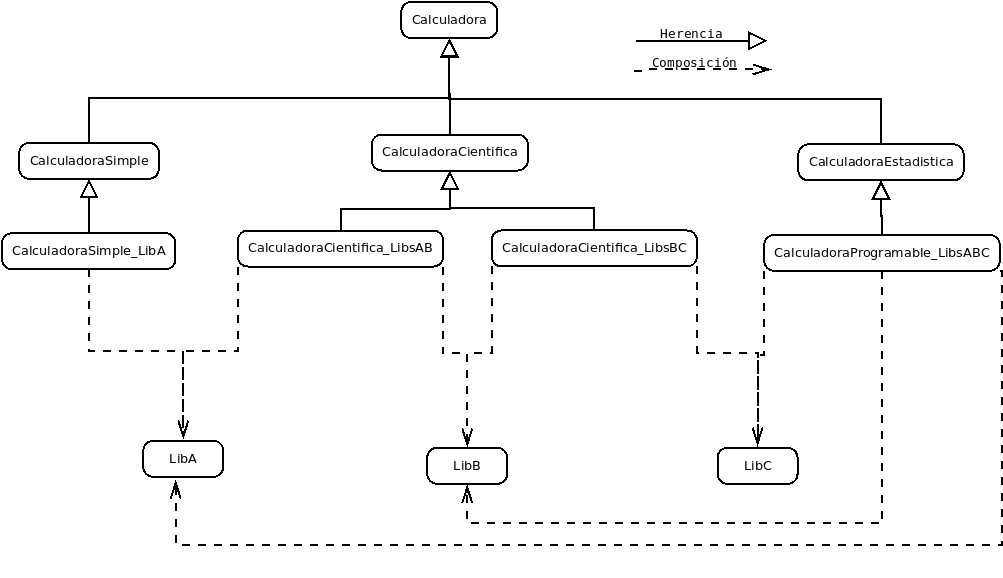
\includegraphics[width=0.99\linewidth]{ej3.png}

\subsection{Punto b}
Si se desea implementar un nuevo tipo de calculadora se debe diseñar un nuevo
módulo abstracto que herede del módulo \textbf{Calculadora} y que provea la interfaz
para cada funcionalidad que ofrezca este tipo de calculadora.
Para agregar una nueva biblioteca o implementar una nueva combinación de tipo
de calculadora y bibliotecas, se debe diseñar un nuevo módulo físico que herede su interfaz
del módulo previamente diseñado para ese tipo y se debe componer con los módulos
de las bibliotecas deseadas.
Por ejemplo, para una calculadora científica que utilice las librerías B y C se debe
diseñar el módulo \textbf{CalculadoraCientifica\_LibsBC} que herede su interfaz del módulo
\textbf{CalculadoraCientifica} y se compone con los módulos \textbf{LibB} y \textbf{LibC}.

\subsection{Punto c}

Primero diseño un módulo abstracto que será un esqueleto de funciones comunes a todas las
calculadoras como encender, apagar, mostrar los resultados, recibir entradas, etc.
En este caso para simplificar solo presento los procedimientos de encender y apagar.

\begin{module}{Calculadora}
\eproc
\proc{encender()}
\proc{apagar()}
\end{module}

Luego, para cada tipo de calculadora diferente diseño un módulo lógico con la interfaz
que provee las funciones correspondiente a cada tipo que se necesite implementar.

\begin{hmodule}{CalculadoraSimple}{Calculadora}
\eproc
\proc{sumar(\eb{Int}, \eb{Int}) : Int}
\proc{restar(\eb{Int}, \eb{Int}) : Int}
\proc{dividir(\eb{Int}, \eb{Int}) : Int}
\proc{mutiplicar(\eb{Int}, \eb{Int}) : Int}
\proc{potenciaDos(\eb{Int}) : Int}
\end{hmodule}

\begin{hmodule}{CalculadoraCientifica}{Calculadora}
\eproc
\proc{sumar(\eb{Int}, \eb{Int}) : Int}
\proc{restar(\eb{Int}, \eb{Int}) : Int}
\proc{dividir(\eb{Int}, \eb{Int}) : Int}
\proc{mutiplicar(\eb{Int}, \eb{Int}) : Int}
\proc{exponenciar(\eb{Int}, \eb{Int}) : Int}
\proc{raizCuadrada(\eb{Int}, \eb{Int}) : Int}
\end{hmodule}

\begin{gmodule}{Lista}{X}
\imp{X}
\eproc
\proc{add(\eb{X})}
\proc{head():X}
\proc{next():X}
\proc{more():Bool}
\proc{delete()}
\end{gmodule}

\cmodule{ListaNumeros}{Lista}{Int}

\begin{hmodule}{CalculadoraEstadistica}{Calculadora}
\imp{ListaNumeros}
\eproc
\proc{sumar(\eb{Int}, \eb{Int}) : Int}
\proc{restar(\eb{Int}, \eb{Int}) : Int}
\proc{dividir(\eb{Int}, \eb{Int}) : Int}
\proc{mutiplicar(\eb{Int}, \eb{Int}) : Int}
\proc{promedio(\e{ListaNumeros}) : Int}
\proc{moda(\e{ListaNumeros}) : Int}
\end{hmodule}

Por último, para cada combinación de tipo de calculadoras y bibliotecas de funciones
matemáticas defino un módulo que herede la interfaz del tipo de calculadora
correspondiente y se compone con los módulos de las bibliotecas que se quieran utilizar

\begin{hmodule}{CalculadoraSimple\_LibA}{CalculadoraSimple}
\imp{LibA}
\end{hmodule}

\begin{hmodule}{CalculadoraCientifica\_LibAB}{CalculadoraCientifica}
\imp{LibA, LibB}
\end{hmodule}

\begin{hmodule}{CalculadoraCientifica\_LibBC}{CalculadoraCientifica}
\imp{LibB, LibC}
\end{hmodule} 

\begin{hmodule}{CalculadoraEstadistica\_LibABC}{CalculadoraEstadistica}
\imp{LibA, LibB, LibC}
\end{hmodule} 



\end{document}